\subsection{Background}
The Corporate Partnership Program is a website designed to `promote the relationship between the Department of Computing and organisations who wish to recruit our students whilst investing in academic sponsorship'\cite{doc-cpp}.

In order for students to use the system they must log on, register some tick box interests, and then upload their CV.
For the student once they have done this their CPP journery is complete.
Corporate Partners then log on and can browse this list of students in order to contact them regarding internships, placements, and graduate oppourtunities.

\begin{center}
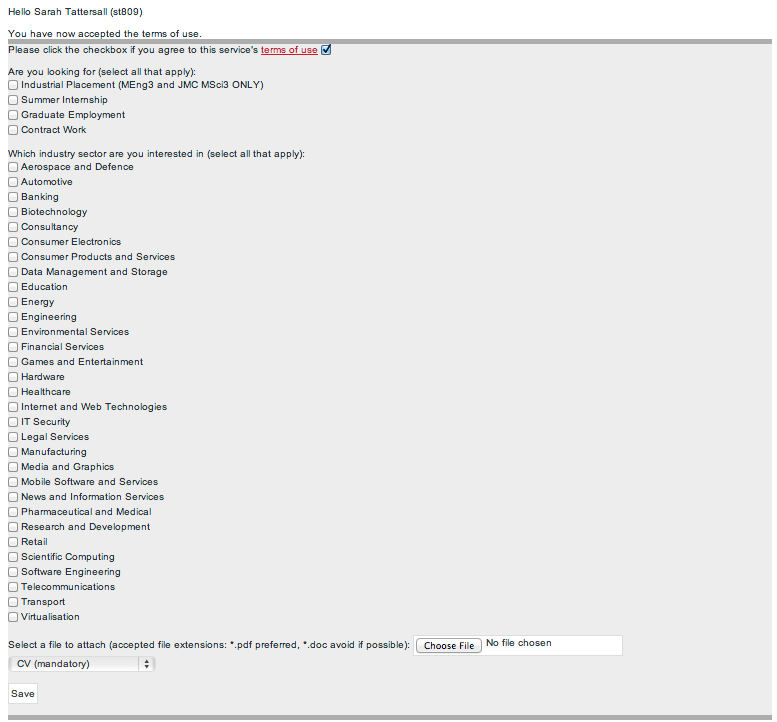
\includegraphics[scale=0.5]{images/introduction/old_cpp}
\end{center}
